\documentclass{lab_sheet}
\usepackage{fancyvrb}
\DefineVerbatimEnvironment{tblCode}{BVerbatim}{baseline=t}
\def\ddfrac#1#2{\displaystyle\frac{\displaystyle #1}{\displaystyle #2}}
\makeatletter
\newcolumntype{v}[1]{>{\topsep=0pt\@minipagetrue\centering\arraybackslash}p{#1}<{\vspace{-\baselineskip}}}
\makeatother
\begin{document}
    \titlePage{Getting Started with MATLAB}{December 5, 2021}
\section{Objectives}
\begin{itemize}
    \item Familiarization and review of basic programming concepts in MATLAB.
\end{itemize}
\section{Background Theory}
\subsection{Variables}
Unlike many programming languages, MATLAB does not require prior definition of the variables, instead the variables can be simply written as,
\begin{verbatim}
    variable name = expression;
\end{verbatim}
For example:
\begin{verbatim}
    a = sin(64) + 2;
\end{verbatim}
If the user doesn't specify the name of the variable, MATLAB automatically creates the
variable \texttt{ans}.   
\begin{verbatim}
    >> 3+2
    ans=5
\end{verbatim}
\subsection{Vectors and Matrices}
Vectors and matrices are used to combine separate scalar data into single, multidimensional signal.
\begin{verbatim}
    >> x=[1:10]
    >> x=[1 3 7 15]
    >> y=[1:0.1:10]
    >> z=[1:3;4:6;7:9]
    >> [m,n]=size(z)
\end{verbatim}
\subsection{Arithmetic Operations}
\begin{itemize}
    \item Arithmetic operators: \verb|+|,\verb|-|,\verb|*|,\verb|/|,\verb|\|,\verb|^| 
    \item Mathematical functions available: \texttt{abs}, \texttt{sqrt}, \texttt{log}, \texttt{sin}, \texttt{cos}
\end{itemize}
\begin{table}[H]
    \centering
    \begin{tabular}{ |c|c| }
        \hline
        \textbf{Mathematical Function}&\textbf{MATLAB Syntax}\\
        \hline\hline
        $f_1=a_1+b_1x+c_1x^2$ & 
        \begin{tblCode}
f1 = a1 + b1*x + c1*x^2
        \end{tblCode}
        \\
        \hline
        $f_2=a_2+b_2x+c_2x^2+d_2x^3$ & 
        \begin{tblCode}
f2 = a2 + b2*x + c2*x^2 + d2*x^3
        \end{tblCode}
        \\
        \hline
        $g=e^{At}\left(C_1\cos(Bt)+C_2\sin(Bt)\right)$ & 
        \begin{tblCode}
g = exp(A*t)*(C1*cos(B*t)+C2*sin(B*t))
        \end{tblCode}
        \\
        \hline
        $u=2xy^2+\sin(x+y)$ & 
        \begin{tblCode}
u = 2*x*y^2 + sin(x+y)
        \end{tblCode}
        \\
        \hline
    \end{tabular}
\end{table}

\subsection{Control Flow}
\begin{table}[H]
    \centering
    \begin{tabular}{ |c|v{3.2cm}|v{3.5cm}|v{3.8cm}| }
        \hline
        \textbf{Loops}&\textbf{FOR Loop}&\textbf{WHILE Loop}&\textbf{IF..ELSE..}\\
        \hline\hline
        \textbf{Syntax}& 
        \begin{verbatim}
for expression
    statements
end
        \end{verbatim}
        &
        \begin{verbatim}
while expression
    statements
end
        \end{verbatim}
        &
        \begin{verbatim}
if expression
    statements
elseif expression
    statements
else
    statements
end
\end{verbatim}
        \\
        \hline
    \end{tabular}
\end{table}
A FOR loop allows a statement to be repeated a fixed, predetermined number of times. The problem is to fill the vector b with square roots of 1 to 1000. One way to do so, is by using a FOR loop. A file named tictoc.m is saved with the following content,
\matlabcode{tictoc}{Matlab script to use tic toc with for loop}
\subsubsection*{Command Window Observation}
\begin{verbatim}
    >> tictoc
    The time required was: 0.000347
\end{verbatim}
\subsection{Different Tasks and Commands}
\subsubsection{User-Defined Functions}
\begin{itemize}
    \item \textbf{Commands:} \texttt{function [op1,op2,...]=cmd\_name(ip1,ip2,...)}
    \item \textbf{Example:}
    \begin{verbatim}
        function y = fcn(x)
            y = sin(x.^2);
        end
\end{verbatim}
\end{itemize}
\subsubsection{Polynomial Roots}
\begin{itemize}
    \item \textbf{Commands:} \texttt{roots(p)}
    \item \textbf{Example:}
    \begin{verbatim}
        >> p = [1 2 1];
        >> r = roots(p)
        r = -1 -1
\end{verbatim}
\end{itemize}
\subsubsection{2D Plotting}
\begin{itemize}
    \item \textbf{Commands:} \texttt{plot, subplot, figure, hold, stem, axis, title}
    \item \textbf{Example:}
    \begin{verbatim}
        >> t=[-2:0.01:2];
        >> x=sin(t*10);
        >> plot(t,x)
        >> axis([-1 1 -1 1])
        >> zoom
        >> xlabel(`Time')
        >> title(`My first plot')
        >> specgram(x)
\end{verbatim}
\end{itemize}
\subsubsection{Dealing with Sound Files}
\begin{itemize}
    \item \textbf{Commands:} \texttt{wavread, wavwrite, auread, auwrite, sound(y,fsamp)}
    \item \textbf{Example:}
    \begin{verbatim}
        >> y=wavread('C:\sound.wav')
        >> sound(y,44100);
\end{verbatim}
\end{itemize}
\subsubsection{Complex Numbers}
\begin{itemize}
    \item \textbf{Commands:} \texttt{j, real, imag, abs, angle}
    \item \textbf{Example:}
    \begin{verbatim}
        >> real(j)       >> imag(j)
        >> abs(j)        >> angle(j)
\end{verbatim}
\end{itemize}
\subsubsection{Signal Processing and
Image Processing}
\begin{itemize}
    \item \textbf{Commands:} \texttt{fft(), dft(), con(), dither(), gray2ind(), ind2gray(), \\ind2rgb(), imread(), imwrite()}
    \item \textbf{Example:}
    \begin{verbatim}
        >> A=imread('my_pic.jpg')
        >> whos
        >> imshow(A)
\end{verbatim}
\end{itemize}
\subsubsection{Transfer Function Representation and Frequency Response}
\begin{itemize}
    \item \textbf{Commands:} \texttt{tf2zp, zp2tf, freqs(), semilogx(), bode()}
    \item \textbf{Example:}
    \begin{verbatim}
        % Given H(s)=(2s+3)(s3+4s2+5)
        >> num=[2 3];
        >> den=[1 4 0 5];
        >> [z,p,k]=tf2zp(num,den);
        >> [num den]=zp2tf(z,p,k);
        >> T=0:0.1:1;
        >> y=step(num,den,t);
        >> plot(t,y)
        >> bode(num,den)
        >> [mag,phase]=bode(num,den,w);
        >> magdb=20*log10(mag);
        >> semilogx(w,magdb)
        >> semilogx(w,phase)
\end{verbatim}
\end{itemize}
\subsection{Getting Help from MATLAB}
\begin{verbatim}
    >> doc fft
    >> help help
    >> help cos
    >> help fft
    >> lookfor filter
\end{verbatim}
\section{Lab Exercises}
\problem{Calculate $\left(1+\ddfrac{2}{n^2}\right)^n$ for n=3, 7}
\matlabcode{lab_1_1}{Matlab function for calculating given polynomial}
\subsubsection*{Command Window Observation}
\begin{verbatim}
    >> lab_1_1(3)              >> lab_1_1(7)
    ans = 1.8258               ans = 1.3232
\end{verbatim}
\problem{Plot the function: $y = e^{-at}cos (\omega t)$, for $a = 2$, $\omega = 5$, and $t = 0:10$.}
\matlabcode{exponential_cosine}{Matlab function to calculate the response for product of exponent and cosine}
\matlabcode{lab_1_2}{Matlab script to plot y for $a = 2$, $\omega = 5$, and $t = 0:10$}
\begin{figure}[H]
    \centering
    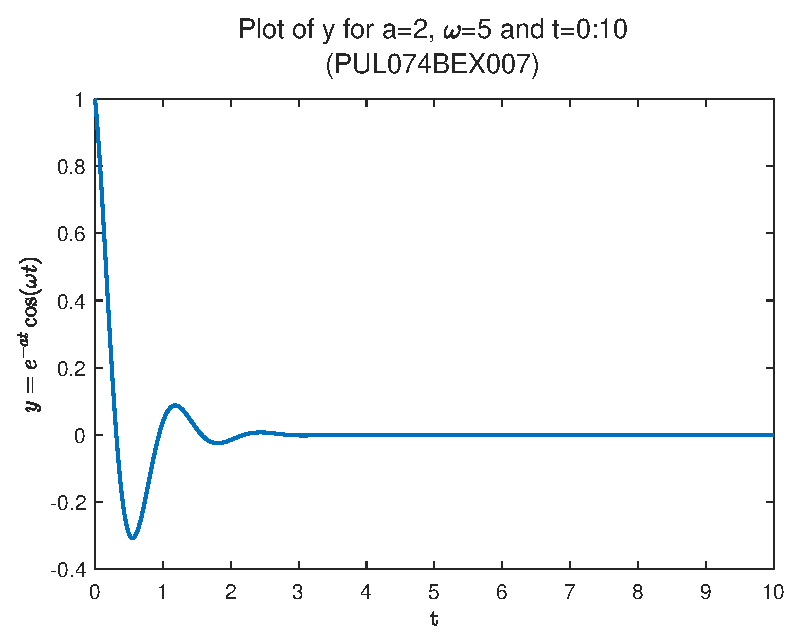
\includegraphics[width=0.9\linewidth]{../Figures/lab_1_2.eps}
    \caption{Plot for $y = e^{-at}cos (\omega t)$ for $a = 2$, $\omega = 5$, and $t = 0:10$}
    \label{fig:1_2}
\end{figure}
\problem{Try using the WHILE and the IF statements to calculate all the Fibonacci numbers so that the sum of two consecutive numbers is smaller than 10,000. How many are even? How many are odd? Try to plot them.}
\subsubsection*{Hints}
\begin{enumerate}
    \item Matlab can increase the size of a vector as it is being created.
    \item To determine whether a number n is even or odd you can use the function \texttt{rem(n,2)}. If
    \texttt{rem(n,2)} equals 0 then the number is even, otherwise it is odd.
\end{enumerate}
\matlabcode{fibonacci_numbers}{Matlab function to return fibonacci numbers within a maximum sum}
\matlabcode{lab_1_3}{Matlab script plot even and odd fibonacci numbers and display their count}
\begin{figure}[H]
    \centering
    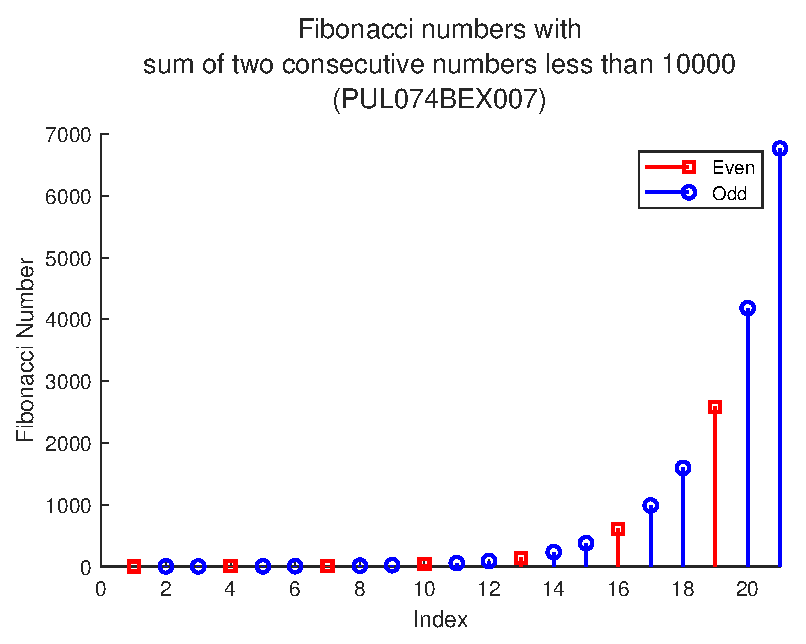
\includegraphics[width=0.9\linewidth]{../Figures/lab_1_3.eps}
    \caption{Plot for fibonacci numbers with sum of two consecutive numbers less than 10000}
    \label{fig:1_3}
\end{figure}
\subsubsection*{Command Window Observation}
\begin{verbatim}
    >> lab_1_3
    Total fibonacci numbers: 21 
    Even fibonacci numbers: 7 
    Odd fibonacci numbers: 14
\end{verbatim}
\problem{Given $f(x)= \ddfrac{x^2+2x+3}{x+3}$. Plot $f(x)$ for $0 \leq x \leq 100$}
\matlabcode{lab_1_4}{Matlab script to plot $f(x)$ for $0 \leq x \leq 100$}
\begin{figure}[H]
    \centering
    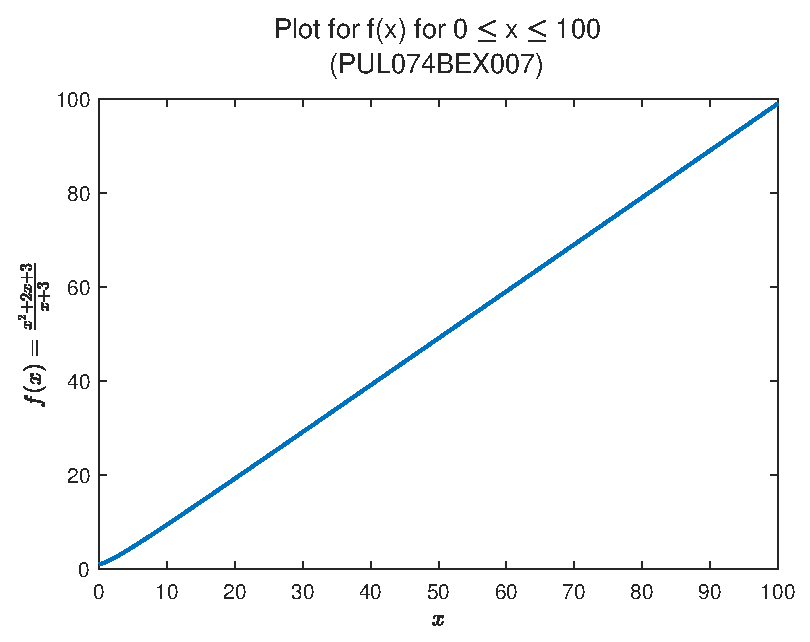
\includegraphics[width=0.9\linewidth]{../Figures/lab_1_4.eps}
    \caption{Plot for $f(x)= \ddfrac{x^2+2x+3}{x+3}$ for $0 \leq x \leq 100$}
    \label{fig:1_4}
\end{figure}
\end{document}